\documentclass[memoire.tex]{subfiles}

\chapter{Concepts formels}

\section{Introduction}
L'objectif de ce chapitre est dans un premier temps de rappeler des notions de probabilités~\cite{probaBio, decision_tree, apprentissage} qui serviront à la compréhension de ce document. Il s'agit ensuite d'expliquer dans sa généralité les concepts d'arbres décisionnels afin d'introduire des principes de classement et d'optimisation.

\section{Rappels de probabilité}
	\subsection{Expérience aléatoire}
Une expérience est dire aléatoire si les résultats possibles sont connus à l'avance sans vraiment savoir celui obtenu au préalable. On appelle univers, noté \(\Omega\), l'ensemble de toutes les issues possibles d'une expérience et \(\omega\) une réalisation de l'expérience.
\begin{equation}
\Omega = \begin{Bmatrix} \omega_1, \omega_2, \cdots, \omega_n \end{Bmatrix}, n \in \mathbb{N}
\end{equation}
		\subsection{Événements}
Un événement correspond à un ensemble de résultats possibles pour une expérience. Si cet ensemble est constitué d'un seul élément, on parle alors d'événement élémentaire. Si l'ensemble de résultats est égal à l'univers \(\Omega\), alors l'événement est dit certain. En revanche, si aucun résultat n'est présent (ensemble \(\emptyset\)), alors c'est un événement impossible.
		\subsection{Probabilités}
Une probabilité est une fonction qui à un événement A, associe un poids.
\begin{equation}
\left \{
\begin{array}{l}
P(\Omega) = 1 \\
P(\emptyset) = 0 \\
0 \leq P(A) \leq 1 \\
P(\bigcup_{i=1}^n A_i) = \sum_{i=1}^n P(A_i)
\end{array}
\right . 
\end{equation}
Plus la probabilité est proche de 1, plus il est possible que l'événement se réalise.
Soit A et B deux événements quelconques, \(P(A)\) est dite conditionnelle si son résultat est influencé par l'événement B :
\begin{equation} 
\left \{
\begin{array}{l}
B \neq \emptyset \\
P(B) \neq 0 \\
A = (A \cap B) \cup (A \cap \overline{B}) \\
\end{array}
\right . 
\end{equation}
On peut alors déduire deux formules : le théorème de Bayes permettant de calculer \(P_B(A)\) et le théorème es probabilités totales qui permet de connaitre la valeur de \(P(A)\) à partir de deux événements A et B. 
\begin{equation}
P_B(A) = \frac{P(A \cap B)}{P(B)}
\end{equation}
\begin{equation}
P(A) = P_B(A)P(B) + P_{\overline{B}}(A)P(\overline{B})
\end{equation}

\section{Arbre de décision}
\subsection{Définition}
Un arbre de décision est une représentation structurelle qui permet d'aboutir à un choix. C'est un graphe acyclique orienté composé :
\begin{itemize}
\item d'un sommet sans parents appelé racine,
\item de sommets appelés nœuds, correspondant à des tests,
\item de sommets terminaux nommés feuilles,
\item des arrêtes, ou branches, désignant chacune les résultats d'un test
\end{itemize}
Pour construire un arbre de décision, une approche \textit{Top-Down} est utilisée, appelée \textit{Top Down Induction of Decision Tree} (\textit{TDIDT}). Elle peut se décomposer en plusieurs parties :
\begin{enumerate}
\item Partir du jeu complet de données et construire la racine.
\item Réaliser un test afin de séparer les données.
\item Séparer le nœud actuel en fonction des résultats possibles.
\item Appliquer récursivement jusqu'à atteindre les feuilles.
\end{enumerate}
Lorsque chaque nœuds sont composés exactement de deux descendants (hors feuilles), on parle alors d'arbre de décision binaire. C'est un cas très largement utilisé des algorithmes de construction d'arbres tels que CART~\cite{ant_colony}, qui sera expliqué ultérieurement.
\subsection{Exemple}
Prenons comme exemple les données météorologiques~\cite{} présente dans la table 1. Cette table est constitué de différentes colonnes concernant différentes information ainsi qu'une colonne indiquant si la décision de sortir a été prise ou non. Dans un peu premier temps, il est possible de déduire les tests à réaliser comme par exemple "La température est-elle élevée ?" ou encore "Quel est le temps ?". A ces questions découlent des réponses possibles, \{oui, non\} pour la première et \{soleil, nuageux, pluie\} pour la deuxième. Une fois l'approche TDIDT utilisée, un arbre de décision est alors obtenu (figure 1.1).

\begin{table}[!h]
\footnotesize
\centering
\renewcommand{\arraystretch}{2}
\begin{tabular}{|c|c|c|c|c|c|}
\hline
% thead
Jour &
Temps & 
Température & 
Humidité & 
Vent & 
Sortie\\
\hline
1  & soleil  & élevée  & haute   & non & N \\
2  & soleil  & élevée  & haute   & oui & N \\
3  & soleil  & moyenne & haute   & non & N \\
4  & soleil  & basse   & normale & non & Y \\
5  & soleil  & moyenne & normale & oui & Y \\
6  & nuageux & élevée  & haute   & non & Y \\
7  & nuageux & basse   & normale & oui & Y \\
8  & nuageux & moyenne & haute   & oui & Y \\
9  & nuageux & élevée  & normale & non & Y \\
10 & pluie   & moyenne & haute   & non & Y \\
11 & pluie   & basse   & normale & non & Y \\
12 & pluie   & basse   & normale & oui & N \\
13 & pluie   & moyenne & normale & non & Y \\
14 & pluie   & moyenne & haute   & oui & N \\
\hline
\end{tabular}
\caption{Table Météo}
\end{table}

\begin{figure}[!h]
	\centering
	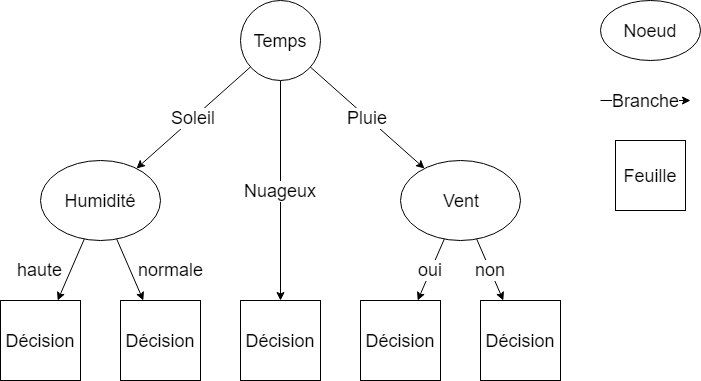
\includegraphics[scale=0.6]{img/decision_tree_meteo.png}
	\caption{Arbre de décision de la table Météo}
\end{figure}

\section{Arbre de décision pour le classement}
		\subsection{Attributs et classes}
Soit un ensemble d'observation \(S\) de taille \(n\):
\[ S = \{s_1, s_2, ..., s_n\}. \]
Chaque observation \(s_i\) est composée d'un ensemble de \(m\) attributs :
\[ A_s = \{a_1, a_2, ..., a_m\}. \]
Soit \(V_j\) l'ensemble de taille \(l\) des valeurs possibles de l'attribut \(a_j\) d'une observation \(s_i\) tels que :
\[ V_j = \{ v_1, v_2, ..., v_l \}. \]
La valeur de l'attribut \(a_j\) sera représentée par \(v_k\).
Un attribut est dit qualitatif si l'ensemble des valeurs possibles est symbolique (non numérique), par exemple si \(V_j\) représente les couleurs d'écriture d'un mot. On obtiendrait alors \( V_j = \{\) bleu, rouge, noir, vert \(\} \).\\

Une donnée est quantitative si l'ensemble des valeurs possibles est un ensemble numérique fini ou infini :
\begin{itemize}
\item Si un attribut peut prendre une infinité de valeurs dans son ensemble, alors celui-ci est qualifié de continu, par exemple le temps d'exécution d'un processus.
\item Dans le cas contraire, une variable dite discrète possède une valeur finie. Elle est généralement liée à une énumération, comme par exemple le nombre de trait dans un caractère. 
\end{itemize}\\

\(a_j\) est nominal si la notion d'ordre n'est pas présente dans l'ensemble des valeurs possibles, par exemple si \(V_j = \{\) un, deux, trois, quatre, cinq, six, sept, huit, neuf \(\} \) représente le nom d'un chiffre en toutes lettres.\\

Un attribut est ordinal si la notion les valeurs possibles contiennent la notion d'ordre. Cela peut être par exemple l'appréciation d'un client : \(V_j = \{\) mauvais, bon, très bon \(\} \)\\

Une variable est qualifiée de binaire si l'ensemble \(V_j\) des valeurs possibles est de taille \(l=2\)\\

La classe d'une observation correspond a une "catégorie" et permet de se rapprocher ou de se différencier des autres observations. Elle correspond à une feuille dans un arbre décisionnel.

		\subsection{Fonction de classement}
		\subsection{Gain d'information}
		\subsection{Entropie}
		\subsection{Information mutuelle}
		\subsection{Apprentissage supervisé}
		\subsection{Exemple}

\section{Arbre de décision pour l'optimisation}
